


%%%%%%%%%%%%%%%%%%%%%%%%%%%%%%%%%%%%%%%%%%%%%%%%%%%%%%%%%%%%%%%%%%%%%%%%%%%%%%%%%%%%%%%%%%%%%%%%%%%%%%%%%%%%%%%%%%%%%%%%%%%%%%%%%%%%%%
%Navrhněte nasazení řešení BYOD. 
\section{Návrh řešení}


\todo{Napsat tomu intro}

%%%%%%%%%%%%%%%%%%%%%%%%%%%%%%%%%%%%%%%%%%%%%%%%%%%%%%%%%%%%%%%%%%%%%%%%%%%%%%%%%%%%%%%%%%%%%%%%%%%%%%%%%%%%%%%%%%%%%%%%%%%%%%%%%%%%%
%Konzultujte navrhované řešení se zástupci vybrané organizace a stanovte doporučení pro nasazení. 
\section{Hodnocení navrhované varianty zástupci KB}\todo{sehnat}




\section{Návaznost na stávající řešení}



\section{Návrh řešení pro notebooky}

KB nehledá komlexní řešení pro virtualizaci pracovních stanic. Stávající situace, kdy zaměstnanci používají firemní zařízení je vyhovující a není důvod do ní jakkoli výrazněji zasahovat. Je však třeba najít odpověď na narůstající trend vlastních zařízení a především představit rámec pro kontraktory, kteří firemním zařízení nedisponují tak, aby nebyli rizikem pro vnitřní síť KB a jejich chování v rámci sítě bylo kontrolováno firemními politikami.

\todo{Návaznost na kapitolu kde analizuju KB BYOD podle prezentace}

Vzhledem k nároků kladeným na BYOD v KB vychází jako řešení nejlépe distribuovaná virtualizace. Navržené řešení umožňuje pokročilou správu distribuovaných virtuálních strojů nutnou pro plnění firemních politik jak ze strany KB, tak i případně ze strany domovské firmy kontraktora.

\subsection{VMware Horizon Flex}
V roce 2014 VMWare představil VMWare řešení VMWare Horizon Flex. Jedná se o kombinaci některých stávajících technologií jako jsou Fusion, Player, Mirage či AirWatch. \todo{citace http://blogs.gartner.com/mark-lockwood/2014/10/14/is-vmwares-horizon-flex-the-answer-to-byod/}. Je odpovědí na požadavky zákazníku provozovat virtuální desktopy offline. Zároveň přináší výhody virtualizace, ale nenese s sebou velké náklady v podobě nutnosti výkonných serverů a dostatečného diskového úložiště jako v případě centralizované virtualizice, což byl jeden s hlavních důvodů, proč centralizovaná virtualizace v KB není rozšířena jako alternativa pro řešení BYOD, viz (\ref{projektVDI}). Nevýhoda virtualizace v podobě vysokých nároků na konektivitu a špatné odezvy je u tohoto řešení taktéž neexistující. 

Uživatelé mohou přistupovat do korporátní sítě z korporátního obrazu operačního systému, ale přitom použivat své vlastní notebooky nebo počítače od firmy Apple, bez toho aby tyto zařízení muselo IT oddělení podporovat. IT může plně spravovat korporátní systém bez toho, aby zasahovalo do operačního systému uživatele. Bezpečnostní rizika jsou minimalizována díky oddělení obou operačních systémů a možnosti vzdáleně řídit omezení pro virtuální stoj, či ho dokonce vzdáleně uzamknout či smazat. Tato možnost je obzvláště výhodné u externích pracovníků, kterým může vypršet kontrakt. Do systému Horizon FLEX je možné zapojit také obrazy virtuálních strojů sloužící pro testování a lépe je tak spravovat.

Technicky se jedná o hypervizor typu 2, který je spravovaný centrálně. Je možné jej nasadit jak pro koncové stanice s Mac OS, tak s Windows. Spravovat, zálohovat a záplatovat systém je též možné centrálně, a to s užitím serveru Mirage for Horizon FLEX. Pro nastavení politik řešení obsahuje Horizon FLEX Policy Server, jako klient je použit VMware Fusion Pro pro počítače Mac a VMware Workstation Player pro počítače s Windows.  \todo{citovat http://www.vmware.com/content/dam/digitalmarketing/vmware/en/pdf/techpaper/vmware-horizon-flex-solution-brief-mirage-fusion-player.pdf} Pro klienta jsou podporovány následující 64bitové operační systémy: Windows 7, Windows 8.1, Windows 10, Mac OS X 10.9, Mac OS X 10.10 a Mac OS X 10.11.

 \begin{figure}[h!]\label{FlexVrstvy}
 \centering
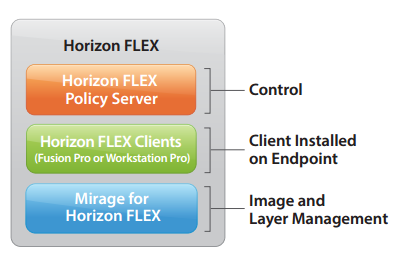
\includegraphics[width=8cm]{img/FlexVrstvy}
\caption{Vrstvy produktu VMWare Horizon FLEX} 
\label{FlexVrstvy}
\end{figure}\todo{citovat http://www.vmware.com/content/dam/digitalmarketing/vmware/en/pdf/techpaper/vmware-horizon-flex-solution-brief-mirage-fusion-player.pdf}



Různě nastavené virtuální stroje je možné distribuovat různým uživatelům. Uživateli musí být nejdříve nainstalován klient a tedy Fusion Pro nebo Workstation Player. Uživatelský systém potřebuje přístup k Horizon FLEX Policy serveru v následujících případech: pro úvodní stažení obrazu stroje a pro získání aktualizací politik a omezení. Horizon Flex Policy Server musí být pro klienta dostupný pomocí https protocol. Je možné nastavit maximální počet dní bez připojení k Policy Serveru. Minimimální hardwarové požadavky serverů jsou sepsány v příloze (\ref{pozadavky})


 \begin{figure}[h!]\label{FlexPolicy}
 \centering
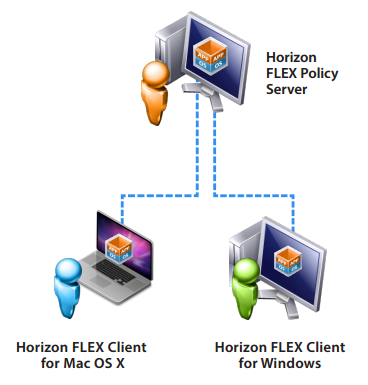
\includegraphics[width=6cm]{img/FlexPolicy}
\caption{Schéma pro připojení k Horizon Flex Policy serveru}
\end{figure}\todo{citovat http://www.vmware.com/content/dam/digitalmarketing/vmware/en/pdf/techpaper/vmware-horizon-flex-solution-brief-mirage-fusion-player.pdf} 


S užitím Policy serveru mohou adminstrátoři mimo jiné spravovat inventář omezených virtuálních strojů, procházet seznam uživatelů a skupin ve službě Active Directory, přiřazovat uživatele a skupiny k jednomu či více virtuálnímu stroji, specifikovat politiky pro dané přiřazení, omezit uživateli přístup k virtuálnímu stroji vzdáleným zamknutím nebo kontrolovat stav virtuálního stroje.

Pro nastavování politik slouží webové uživatelské rozhraní. Je možné nastavit následující omezení:

\begin{itemize}
    \item Expirační doba -- Doba, po kterou je virtuální stroj přístupný.
    \item Použití USB zařízení -- Blokování použití zvolených USB zařízení.
    \item Copy\&Paste operace -- Omezení funkce copy and paste mezi hostitelským a virtualizovaným operačním systémem.
    \item Drag\&Drop operace -- Omezení drag and drop funkcionality mezi hostitelským a virtualizovaným operačním systémem.
    \item Zadaní hesla pro kopírování či přesouvání virtuálního stroje.
    \item Omezení existujících instancí virtuálního stroje na jednu.
    \item Omezení možnosti přidělování hardwarových prostředků pro virtuální stroj.
\end{itemize}

Virtuální stroj je též možné vzdáleně uzamknout a nebo smazat.

\section{Návrh nasazení řešení WMware Horizon FLEX}
\todo{citovat http://www.vmware.com/content/dam/digitalmarketing/vmware/en/pdf/techpaper/vmware-horizon-flex-deployment-considerations.pdf}

V první řadě je třeba vyhradit prostor na kterém budou umístěny obrazy pro virtuální stroje. Je vhodné připravit souborové servery pomocí IIS a to jeden uvnitř podnikové sítě a jeden vně. Dále je potřeba nainstalovat Mirage Management server a jeho komponenty. Při zadání sériového čísla se zpřístupní funkce pro Horizon FLEX. 

Jelikož v prostředí KB se používá operační systém Windows, pro vytvoření obrazu pro virtuální stroj je potřeba použít nástroj VMware Workstation Pro, viz. obrázek \ref{workstation}

\begin{figure}[h!]\label{workstation}
\centering
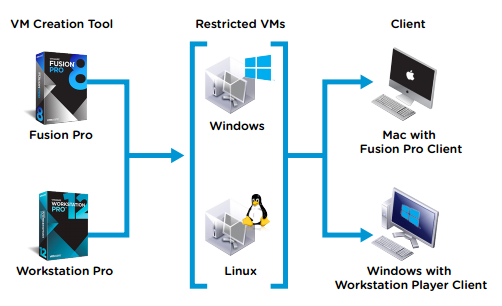
\includegraphics[width=10cm]{img/workstation}
\caption{Schéma postupu pro vytvoření obrazu virtuálního stroje}

\end{figure}\todo{citovat http://www.vmware.com/content/dam/digitalmarketing/vmware/en/pdf/techpaper/vmware-horizon-flex-deployment-considerations.pdf} 




\begin{figure}[h!]\label{schemaArchitektury}
\centering
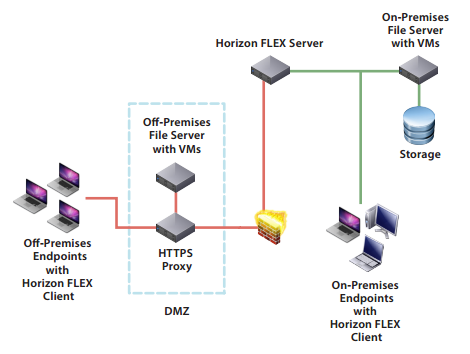
\includegraphics[width=10cm]{img/schemaArchitektury}
\caption{Doporučené schéma infrastruktury pro nasazení VMware Horizon FLEX}
\end{figure}\todo{citovat http://www.vmware.com/content/dam/digitalmarketing/vmware/en/pdf/techpaper/vmware-horizon-flex-deployment-considerations.pdf} 


Po instalaci serveru Mirage je třeba nainstalovat nainstalovat ostatní komponenty Horizon FLEX, nastavit certifikáty pro virtuální stroje, vytvořit a přiřadit virtuální stroje a nakonec nainstalovat klienty na koncová zařízení. Klienty je možné distribuovat uživatelům s připravenými virtuálními stroji. 

Jelikož jeden Horizon FLEX Server dokáže obsloužit až 10000 uživatelů, bude pro potřeby KB stačit pouze jeden server. 



\section{Návrh řešení pro mobilní zařízení}

Z analýzy požadavků uživatelů vyplynulo, že pro mobilní telefony je požadována především dostupnost emailu a pro tablety je to především dostupnost emailu, dokumentů a PIM. Z hlediska požadavků bussinesu je to vzhledem k povaze bankovního sektoru především vysoká bezpečnost.

Přestože leaderem trhu EMM je řešení AirWatch od společnosti VMware, v klíčových vlastnostech pro KB není nejsilnější. VMware je vysoce modulární řešení schopné plnit vysoké nároky. Jeho slabou stránkou je PIM, kde je doporučeno použít řešení od třetí strany.

V klíčových požadavcích exceluje řešení od společnosti BlackBerry. Pro email a PIM nabízí kvalitní produkt BlackBerry Work. V oblasti bezpečnosti je společností Gartner hodnocen jako nejlsilnější hráč na trhu \todo{citace https://www.gartner.com/doc/reprints?id=1-3GSO3TQ\&ct=160902\&st=sb}.

\begin{figure}[h!]\label{GartnerBB}
\centering
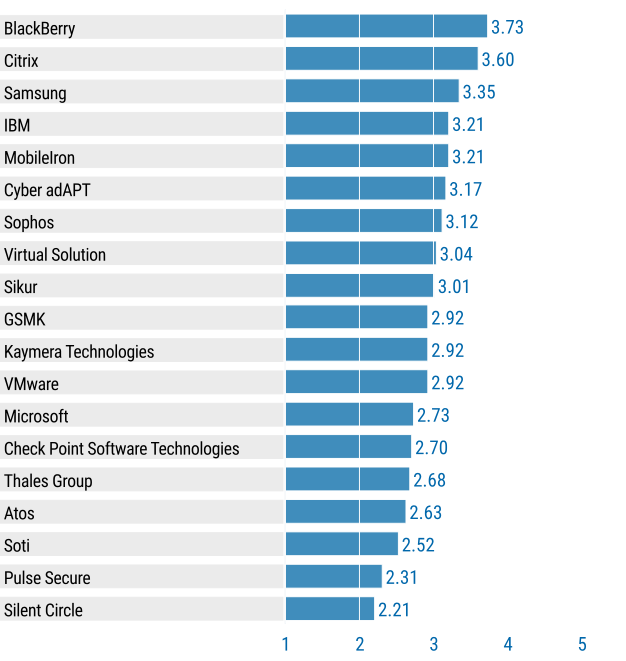
\includegraphics[width=10cm]{img/GartnerBB}
\caption{Hodnocení dodavatelů software pro vysoce bezpečnou správu mobilních zařízení v kategorii BYO od spole4nosti Gartner}
\end{figure}\todo{citovat https://www.gartner.com/doc/reprints?id=1-3GSO3TQ\&ct=160902\&st=sb} 

Společnost Gartner hodnotila produkt v několika kategoriích. 

Z hlediska certifikací a ocenění je situace rozdílná pro každou aplikaci v balíku. Good Dynamics je certifikován jako EAL4+. Kryptografické komponenty jsou certifikovány jako FIPS 140-2 Level 1. Mezi další certifikace, které splňují komponenty od Good technologies patří například ISO 19790 či další státní a armádní normy.

Co se týče MDM funkce nabízí BlackBerry všechny běžné funkce. Platforma podporuje Android for Work i Samsung Knox. Kontejnerizaci aplikací zajišťuje komponenta Good Dynamics. Je možné chránit aplikace hesly a přiřazovat jim certifikáty. Kontejnery mezi sebou mohou komunikovat s užitím certifikátů podepsaných backendovým serverem. 


Dalším důvodem pro volbu BlackBerry je použití tohoto řešení v mateřské firmě Société Générale. Během analýzy bylo zjištěno, že toto řešení se připravuje také pro KB a že během vypracovávání této diplomové práce začala fáze plošného nasazování. Jelikož je řešení od BlackBerry podle analýzy požadavků v této práci nejvhodnějším řešením, tato práce nasazení zvoleného řešení podporuje. Řesení je integrovatelné s řešením od různých poskytovatelů NAC včetně řešení od Cisca.    

Nejdůležitější komponentou pro potřeby KB je BlackBerry Work. Dle specifikací \todo{citovat https://ca.blackberry.com/enterprise/gfe-comparison} nabízí následující funkcionalitu:

Email:
\begin{itemize}
    \item Synchronizace emailu
    \item Správa emailu
    \item Zabezpečené zobrazování příloh
    \item Správa fotografií
    \item Vyhledávání emailů na serveru
    \item Prioritizace oznámení
    \item Inegrace s nositelnostmi
\end{itemize}

Kalendář:
\begin{itemize}
 \item Synchronizace kalendáře
 \item Připojení ke konferenčním hovorům
 \item Plánuvání meetingů
 \item Zprávy "mimo kancelář"
 \item Zobrazení přijatých pozvánek
\end{itemize}

Kontakty:
\begin{itemize}
   \item Synchronizace kontaktů
   \item Vyhledávání v pracovních kontaktech přímo z telefonu
   \item Historie zpráv
\end{itemize}

Kolaborace:
\begin{itemize}
   \item Ukládání souborů do repozitáře
   \item Zabezpečený prohlížeč pro přístup k firemnímu intranetu
   \item Správa úkolů
   \item Přístup k dokumentům ve službách SharePoint, OneDrive nebo Box
   \item Prezentační mód pro prezentaci PowerPoint dokumentů
\end{itemize}

Zajímavou funkcí je jednoduchý přístup pomocí funkce Touch ID na zařízeních s operačním systémem iOS podporující funkci Touch ID.\\

Možnoti administrace:
\begin{itemize}
   \item Šifrovaný kontejner
   \item Integrované MDM
   \item Jednotný dokumentový server
   \item Integrované MAM
   \item Použití technologie Exchange ActiveSync
   \item Rozdělení účtování dat na pracovní a soukromý provoz
\end{itemize}

\subsection{Návrh licencování}

Nejnutnější funkce pro splnění požadavků předpokládaných uživatelů BYOD splňuje komponenta BlackBerry Work. Ta je součástí skupiny služeb BlackBerry Dynamics. Aplikace BlackBerry Dynamics se licencují pouze jako součást balíku Blackberry Enterprise Mobile Suites, který je nabízen v různých edicích.

Pro splnění požadavků na funkce emailu je postačuje edice BlackBerry Enterprise Mobility Suite --  Enterprise Edition. Pro pokročilejší práci s dokumenty vyžadovanou pro BYOD tablety je třeba zakoupit vyšší edici BlackBerry Enterprise Mobility Suite -- Collaboration Edition, viz \todo{ citovat datasheet https://global.blackberry.com/content/dam/blackberry-com/PDF/enterprise/ds-blackberry-enterprise-mobility-suite.pdf}. Tato vyšší edice je též třeba pro integraci s IM klientem Skype for Bussiness.

Tato edice nabízí následující typy aktivace: Work and personal - Regulated, Work space only, Work and personal - user privacy (Android for Work -- Premium), Work space only (Android for Work - Premium), Work and personal - user privacy (Samsung KNOX), Work and personal - full control (Samsung KNOX), Work space only (Samsung KNOX). Nabízí tedy vhodné možnosti jak pro BYOD zařízení, tak pro správu firemních zařízení. 

Pro BYOD mobilní telefony s operačním systémem Android je tedy vhodná licence BlackBerry Enterprise Mobility Suite -- Enterprise Edition a typ aktivace Work and personal -- user privacy.

Pro BYOD mobilní telefony s operačním systémem iOS je vhodná licence BlackBerry Enterprise Mobility Suite -- Enterpirse Edition a typ aktivace user privacy.

Pro BYOD tablety s operařním systémem Android je nejvhodnější licence BlackBerry Enterprise Mobility Suite -- Collaboration Edition a typ aktivace Work and personal - user privacy (Android for Work - Premium).

Pro BYOD tablety s operačním systémem iOS je nejvhodnější licence BlackBerry Enterprise Mobility Suite -- Collaboration Edition a typ aktivace User privacy.

Pro všechny BYOD užití je vhodnější serverový typ licence.

Informace o licencování byly čerpány z oficiální dokumentace \todo{citovace http://help.blackberry.com/en/blackberry-uem/12.6/licensing/dhd1465315353877.html}.


\section{Návrh nasazení řešení pro mobilní zařízení}

\subsection{Komponenty řešení}


Základním kamenem řešení je BlackBerry Unified Endpoint Management (UEM).\todo{cituju http://help.blackberry.com/en/blackberry-uem/current/} Jedná se o infrastrukturu pro zajištění MDM. BlackBerry Infrastructure je vnější server, který spravuje informace o zařízení jako jsou licence a šifrovaně komunikuje s UEM a také s koncovými zařízeními.

\begin{figure}[h!]\label{BBUEM1}
\centering
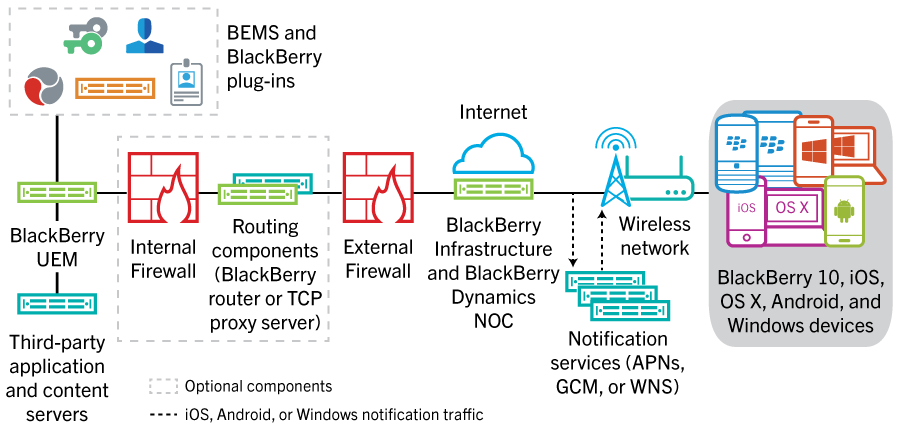
\includegraphics[width=12cm]{img/BBUEM1}
\caption{Architektura BlackBerry UEM}
\end{figure}\todo{citovat http://help.blackberry.com/en/blackberry-uem/current/} 

Pro potřeby splnění požadavků na BYOD je potřeba nasadit další komponenty balíku BlackBerry Enterprise Mobile Suite na úrovni edice Collaboration Edition. Na obrázku \ref{BBEMS} jsou jednotlivé komponenty rozkreslené.

\begin{figure}[h!]\label{BBEMS}
\centering
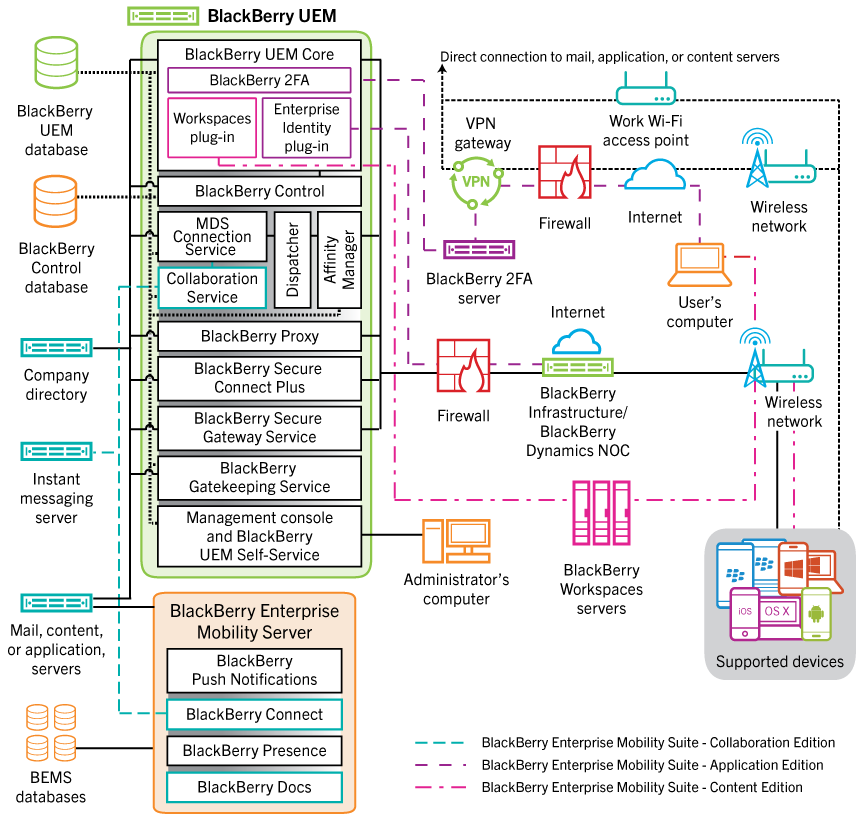
\includegraphics[width=13cm]{img/BBEMS}
\caption{Schéma komponentů balíku BlackBerry Enterprise Mobility Suite}
\end{figure}\todo{citovat http://help.blackberry.com/en/blackberry-enterprise-products/latest/enterprise-products/eqg1459529064051.html} 

Jádrem řešení je BlackBerry UEM, který dále obsahuje subkomponenty jako jsou mimo jiné logování, monitoring, reportování, funkce pro správu, služby pro autentifikaci a autorizaci, plánování a zasílání příkazů či IT politiky a profily zařízení. BlackBerry Control služí k zasílání konfiguračních dat do aplikací BlackBerry Dynamics v koncových zařízeních. BlackBerry Collaboration Service poslouží k propojení se službou Microsoft Skype For Business. 

BlackBerry Enterprise Mobility Server slouží k posílání dat do BlackBerry Dynamics Apps. Většina funkcí je využitelná až u vyšších edicí BlackBerry Enterprise Mobility suite.

\subsection{Kroky instalace}
V první řadě je třeba nainstalovat BlackBerry UEM. Dále je třeba nainstalovat BlackBerry Enterprise Mobility Server. V rámci tohoto severu je třeba nakonfigurovat BlackBerry Dynamics a nastavit certifikáty.  Dále je třeba nastavit přístup do Active directory, SMTP server a Exchange ActiveSync. Dalším krokem je nastavení konektivity pro BlackBerry Dynamics. Po té je nutné nastavit BlackBerry Dynamics profil a zpřístupnit tak uživatelům aplikace BlackBerry Work a BlackBerry Access. 

V BlackBerry dynamics je možné nastavit některé politiky. Pro účely BYOD zařízení je třeba nastavit zamezení přístupu uživatelům s operačním systémem umožnující administrátorské operace (JailBreak/Root) a nastavit interval nutný pro synchronizaci s UEM.

Posledním krokem je nastavení uživatelských účtů a skupin. Aktivace z hlediska uživatele spočívá v instalaci software BlackBerry UEM a BlackBerry work z obchodu s aplikacemi pro svůj operační systém. Další postup aktivace je triviální.

\subsection{Integrace s Cisco ISE}

\todo{todle vsecko cituju z manualu http://help.blackberry.com/en/blackberry-uem/12.6/}

BlackBerry UEM je možné integrovat s Cisco ISE, čož je NAC prvek používaný v KB. Díky této integraci ISE může od UEM získávat data o zařízení, na základě kterých může povolit nebo zamítnout přístup zařízení do firemní sítě.

Cisco ISE vyžaduje v UEM vlastní administrátorský profil, ten je třeba nastavit. Dále je třeba importovat do ISE BlackBerry Web Service Certificate exportovaný z UEM. V ISE je nyní možné nastavit připojení k UEM. 

Nyní může ISE získávat data o zařízení jako je MAC adresa, splnění politik, nastavení šifrování, informace o aktivaci v UEM, detekce jailbreak, výrobce, model, sériové číslo, verze operačního systému, nastavení zaheslování.

Dále je díky integraci přímo z ISE možné vymazat ze zařízení pracovní data nebo jej uzamknout.

\todo{obr ISE str 366}


Maximální počet uživatelů na jeden server 20 000, což znamená, že KB bude stačit jediný server. 

\todo{Nasazeni - Cisco guide}
\todo{Nasazeni - Cisco Good Integration}


\todo{Návrh dalších opatření}
\todo{nastavení pravidel}
\todo{určení kompenzací zaměstnanci vs kontraktoři}
\todo{zákazy, směrnice smlouva}


%Zhodnoťte uskutečnitelnost řešení a analyzujte benefity a rizika spojená se zavedením navrženého konceptu.
\section{Analýza navrženého řešení}